\section{Primera captura: Laboratorio de Pabellón 1}

\par Para una primera experimentación, decidimos correr la herramienta sniffer en la red interna del pabellón 1 de Ciudad Universitaria. Nos conectamos por Wifi a la red y tomamos muestras durante 17 minutos. Utilizamos la fuente de información S1 para diferenciar cada host como un símbolo. Luego, calculamos la información de cada host y con esto, la entropía de la fuente (red).

\subsection{Resultados y análisis}

\par En el gráfico \ref{fig:exp1_labo_infovsentro} se pueden ver los 25 hosts con menor información. La linea punteada roja representa la entropía de la fuente y, como se observa rápidamente, hay un solo host que se encuentra del lado izquierdo (\textbf{10.210.210.199}). Esto significa que es un símbolo con muy poca información y por ende, mucha probabilidad. Para nosotros, esto significa que es un host que participa mucho de la red, preguntando constantemente qué dirección MAC corresponde a una dirección IP. Tomamos entonces a este host como un nodo distinguido de la red.

\begin{figure}[h]
  \begin{subfigure}{.5\textwidth}
    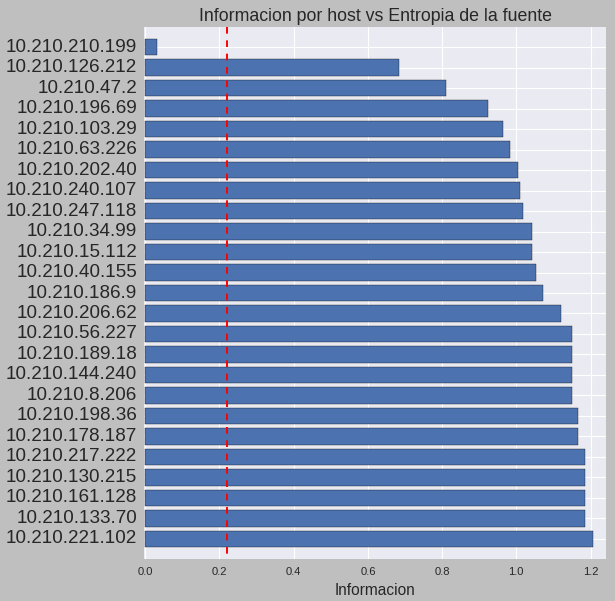
\includegraphics[width=\textwidth]{imagenes/laboratorio/informaciones_vs_entropia.png}
  \end{subfigure}
  \label{fig:exp1_labo_infovsentro}
  \caption{Información de cada símbolo (host) de la red comparada con el valor de la entropía de la fuente de información (red local). Se limita el gráfico a los 25 símbolos con menor valor de información.}
\end{figure}

\begin{figure*}[ht]
  \hspace*{-0.5cm}
  \begin{subfigure}{1.1\textwidth}
    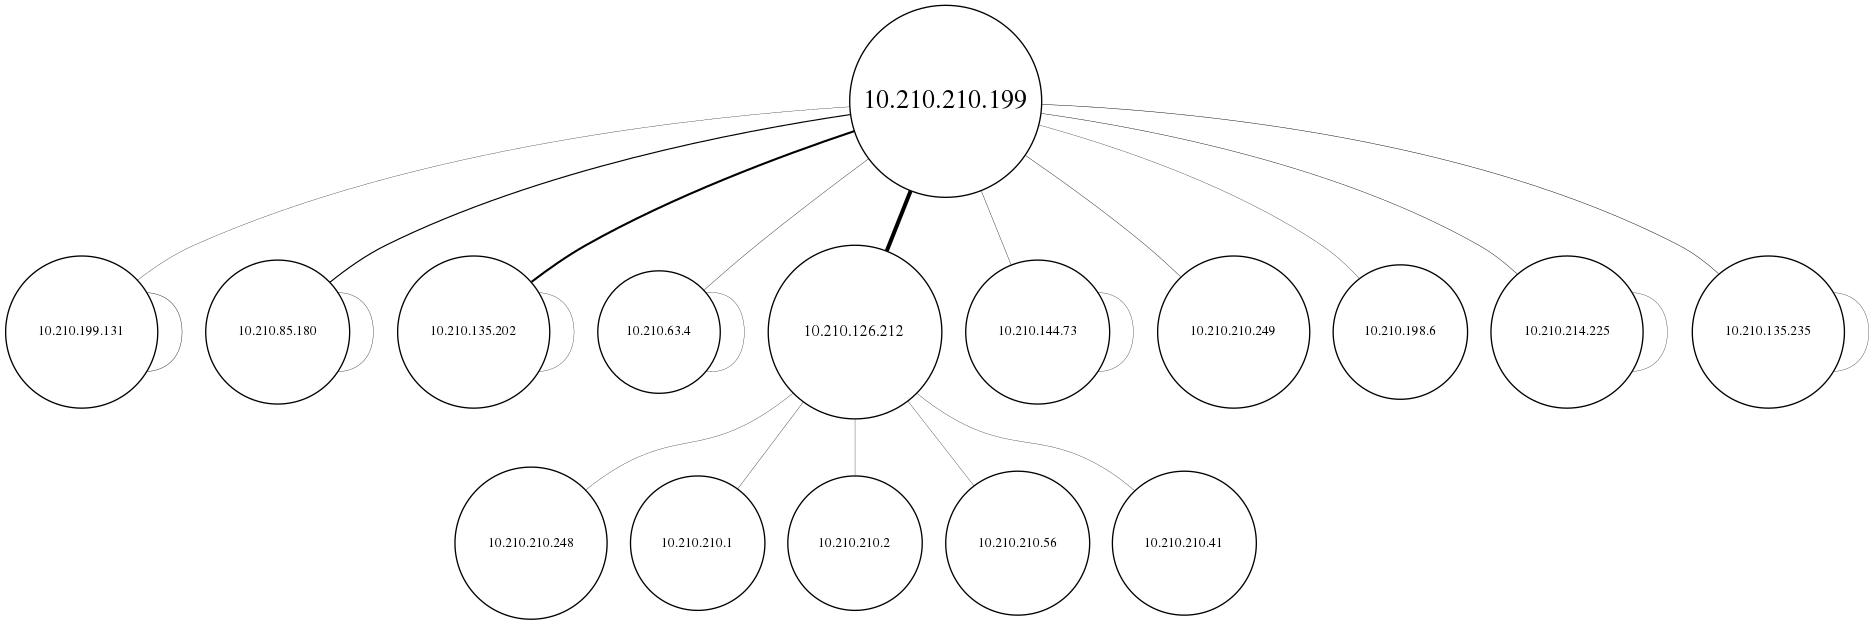
\includegraphics[width=\textwidth]{imagenes/laboratorio/grafo_10.png}
  \end{subfigure}
	\label{fig:exp1_labo_grafo}
	\caption{Grafo con los nodos mas interesantes de la red de la primer captura. El diámetro del nodo implica mayor participación.}
\end{figure*}

\par La distinción del host con IP \textbf{10.210.210.199} la podemos corroborar en el gráfico de la figura \ref{fig:exp1_labo_grafo}. Este grafo representa a la red relacionando nodos con hosts y aristas con mensajes. El diámetro de los nodos está dado por el nivel de participación que tiene en la captura tomada. Asimismo, se obviaron muchos nodos con comportamiento similar que no sumaban valor al grafo, asegurando que los mas \textit{participativos} se mantengan. Este valor de \textit{participación} fue calculado teniendo en cuenta los siguientes parámetros:

\begin{enumerate}
	\item Cantidad de mensajes ARP enviados (solo tomando los del tipo who-has).
	\item Cantidad de mensajes ARP que consultaban por su ip (solo tomando los del tipo who-has).
	\item Cantidad de hosts \textit{distintos} por los cuales preguntó su dirección MAC.
	\item Cantidad de hosts \textit{distintos} que preguntaron por su dirección MAC.
\end{enumerate}

\par A estos 4 parámetros se les asigna un peso, que depende de lo que queramos observar. En este caso en particular, los parámetros 1 y 2 tienen peso 0 porque queríamos enfocarnos en los 3 y 4, que en cierta forma implican a los 1 y 2 (si la cantidad de \textit{distintos} es grande, esto implica que la cantidad sin tener en cuenta distinción de hosts también es grande). Al parámetro 3 le asignamos peso 2, mientras que al 4 le asignamos peso 10. De esta manera, podemos destacar fuertemente los hosts por los cuales muchos otros consultaron por él, pero también teniendo en cuenta (con menor importancia) los hosts que consultaron por muchas direcciones. Lo que logramos con estos valores, es lo que observamos en el grafo de la figura \ref{fig:exp1_labo_grafo}.
\par Las aristas por su parte, representan la consulta de un host por la dirección MAC de otro (sin diferenciar la dirección de los mensajes). Y el peso de cada arista (relacionado con el grosor) está dado por la cantidad de mensajes que relacionan a los hosts.
\par Observando este grafo, notamos que el host con IP \textbf{10.210.126.212} tiene un comportamiento particular. Para analizar mejor la situación vamos a referirnos al host con IP \textbf{10.210.210.199} como \textbf{Nodo A} y al host con IP \textbf{10.210.126.212} como \textbf{Nodo B}. A continuación vamos a mencionar información que extrajimos de la muestra y luego pasaremos a analizar el por qué de estos valores y tratar de caracterizar los nodos según su comportamiento:

\begin{itemize}
  \item Solo el nodo A preguntó por la dirección del nodo B, y lo hizo 121 veces.
  \item El nodo B nunca preguntó por la dirección del nodo A, mientras que otros 268 hosts si lo hicieron.
  \item El nodo A realizó 5796 preguntas, por 298 direcciones distintas (entre ellas la ip del nodo B).
  \item El nodo B realizó 151 preguntas, por 101 direcciones distintas.
\end{itemize}

\begin{figure}[h]
  \begin{subfigure}{.5\textwidth}
    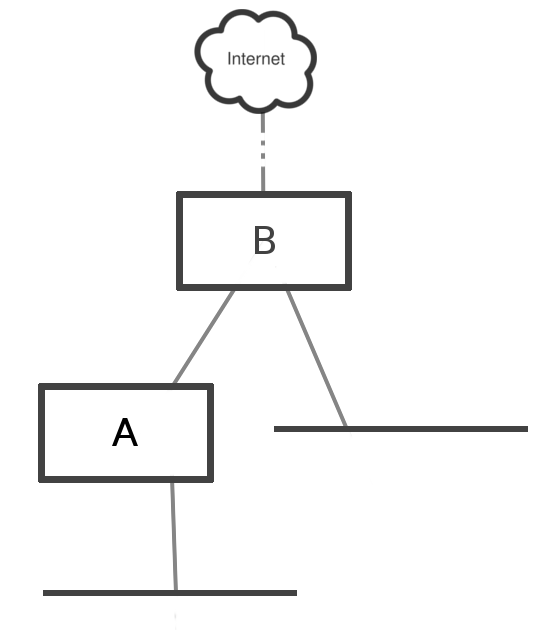
\includegraphics[width=\textwidth]{imagenes/laboratorio/red.png}
  \end{subfigure}
  \label{fig:exp1_labo_red}
  \caption{Diagrama de cómo creemos que está organizada la red de la primera captura.}
\end{figure}

\subsection{Conclusiones}

\par Por esta información, creemos que el nodo A es un access point de la red Wifi, ya que tiene interacción con muchos hosts (entre 268 y 297) y la gran mayoría de ellos solo preguntan por él. Y en el caso del nodo B, creemos que es algún router por el cual debe acceder el nodo A para poder salir a internet. Al mismo tiempo, el nodo B tiene interacción con bastantes hosts (151). También vemos que no tienen interacciones en común (quienes preguntan por A no preguntan por B, y la inversa). Por esto, creemos que el nodo B debe ser el gateway de otra red local. En la figura \ref{fig:exp1_labo_red} planteamos la idea de lo que creemos que puede ser la red, dejando varios interrogantes, pero dando una idea general de su organización.

\\
\newpage
